\documentclass[8pt]{article}

\usepackage{amsmath,listings,graphicx,caption,subfig,float}
\usepackage[margin=0.5in]{geometry}

\begin{document}

\noindent
Robert Werthman\\
CSCI 5622\\
Homework 1: Logistic Regression\\

\begin{enumerate}
\item \textbf{How did the learning rate affect the convergence of your SGA implementation?}\\
The goal of the SGA implementation is to maximize the log-likelihood function.  When we talk about convergence we are talking about reaching the maximum of the log-likelihood function.  The graph below was produced with different constant learning rates $\eta$ with 10 passes through the training set for each learning rate.  As can be seen in the graph, the smaller the learning rate $\eta$, the slower the log-likelihood function value converges to its maximum.  The larger learning rates don't look like they converge to the maximum at all.\\
\begin{center}
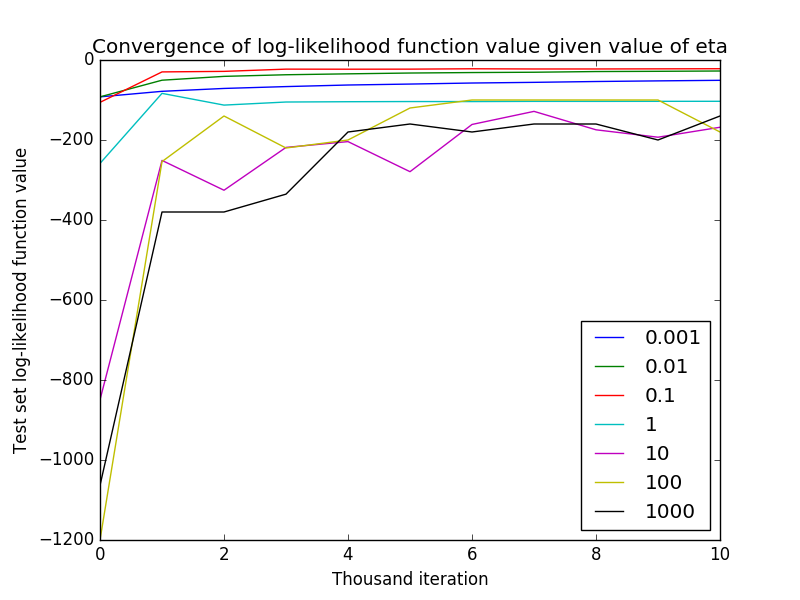
\includegraphics[scale=.3]{q1.png}
\end{center}
\item \textbf{What was your stopping criterion and how many passes over the data did you need to complete before stopping?}\\
If I didn't see the log-likelihood function value increasing or the value was jumping around and never converging to the maximum value, then I would stop the logistic regression.  This depended on the value of $\eta$.  As was talked about in question 1, some values of $\eta$ don't seem to converge or converge very slowly.  This requires more or fewer passes through the data to maximize the log-likelihood function.  When testing, I used 10 passes through the data, but it looked like for some values of $\eta$, more or fewer passes would've gotten the same or better value for the log-likelihood function.  

\item \textbf{What words are the best predictors of each class? How (mathematically) did you find them?}\\
The words that have the highest positive weights when the class is positive at the end of running logistic regression are the best predictors of the positive class.  The words that have the highest negative weights when the class is negative at the end of running logistic regression are the best predictors of the negative class.  These weight distinctions produce the largest log-likelihood function value for each class based on the log of the value returned by the sigmoid function.  This is discussed more in question 4.
\begin{figure}[H]
\centering
\subfloat[Postive Class (Baseball) Best Predictors]{
\begin{tabular}{|c|c|}
\hline
Word & Weight \\
\hline
runs & 1.84356157307\\
guy & 1.80428359188\\
hit & 1.79183652188\\
baseball & 1.45275289035\\
long & 1.31152306307\\
\hline
\end{tabular}}
\hspace{1cm}
\subfloat[Negative Class (Hockey) Best Predictors]{
\begin{tabular}[h]{|c|c|}
\hline
Word & Weight \\
\hline
popped & -6.2896482661\\
best & -3.14376300768\\
coverage & -2.30323451703\\
final & -2.23644919701\\
home & -2.06672434882\\
\hline
\end{tabular}}
\end{figure}
\item \textbf{What words are the poorest predictors of classes? How (mathematically) did you find them?}\\
The poorest predictors of the baseball (positive) class are the words that are the best predictors of the hocky (negative) class, and vice versa.  This is due to the fact that when the log-likelihood function values are calculated, if the weights are high, than the sigmoid function will return a higher value.  If the class is positive than the the log-likelihood value is just the log of that returned value. If the class is negative then the log-likelihood value is the log of 1 minus that returned value.  In both cases, to maximize the value returned by the log of something, you need to give it the highest input value possible.  In the case of the positive class, this is a postive weight; in the case of the negative class, this is a negative weight.

\end{enumerate}

\end{document}